\usepackage{etex} %эта магическая херь избавляет от переполнения регистров TeX а!!!

\mode<article>{\usepackage{fullpage}}
\mode<presentation>{
    \usetheme{Madrid}
    \useoutertheme{shadow}
} 

\usepackage[utf8]{inputenc}
\usepackage[russian]{babel}
\usepackage{indentfirst}
\usepackage{graphicx}

\usepackage{amsmath}
\usepackage{amsfonts}
\usepackage{amsthm}
%\usepackage{algorithm}
%\usepackage{algorithmic}

%\usepackage[all]{xy}

\date{Лекция по дисциплине <<методы и средства защиты компьютерной информации>> (\today)}
\author[М.~М.~Шихов]{Михаил Шихов \\ \texttt{\underline{m.m.shihov@gmail.com}}}

%%для рисования графов пакетом xy-pic
%\entrymodifiers={++[o][F-]}

%%для псевдокода алгоритмов (algorithm,algorithmic)
%\renewcommand{\algorithmicrequire}{\textbf{Вход:}}
%\renewcommand{\algorithmicensure}{\textbf{Выход:}}
%\renewcommand{\algorithmiccomment}[1]{// #1}
%\floatname{algorithm}{Псевдокод}

%\setbeamercolor{alerted text}{fg=-green} %gyan, blue, green, -green

\title[Помехоустойчивое кодирование]{Защита целостности. Помехоустойчивое кодирование. Линейные блоковые коды}


\begin{document}


\mode<article>{\maketitle\tableofcontents}

\frame<presentation>{\titlepage}
\begin{frame}<presentation>[allowframebreaks]
    \frametitle{Содержание}
    \tableofcontents
\end{frame}


\section{$(n,k)$ линейный блоковый код}


\subsection{Целостность}


\begin{frame}
    \frametitle{Свойство целостности}
    
    \begin{definition}
        \alert{Целостность} информации --- это её неизменность относительно некоторого фиксированного значения.
    \end{definition}
    Например, это свойство дает \alert{получателю} уверенность в том, что он получил информацию в том виде, 
    в котором она была отправлена \alert{источником}. 
    
    В любом канале передачи информации имеется \alert{шум} (источник \alert{помех}), который воздействует 
    на передаваемый \alert{сигнал}, искажая его. 
    
\end{frame}


Рассмотрим схему канала передачи информации, представленную на


\begin{frame}
    \frametitle{Схема канала передачи данных}
    
    \begin{figure}
        \begin{center}
            \mode<presentation>{ 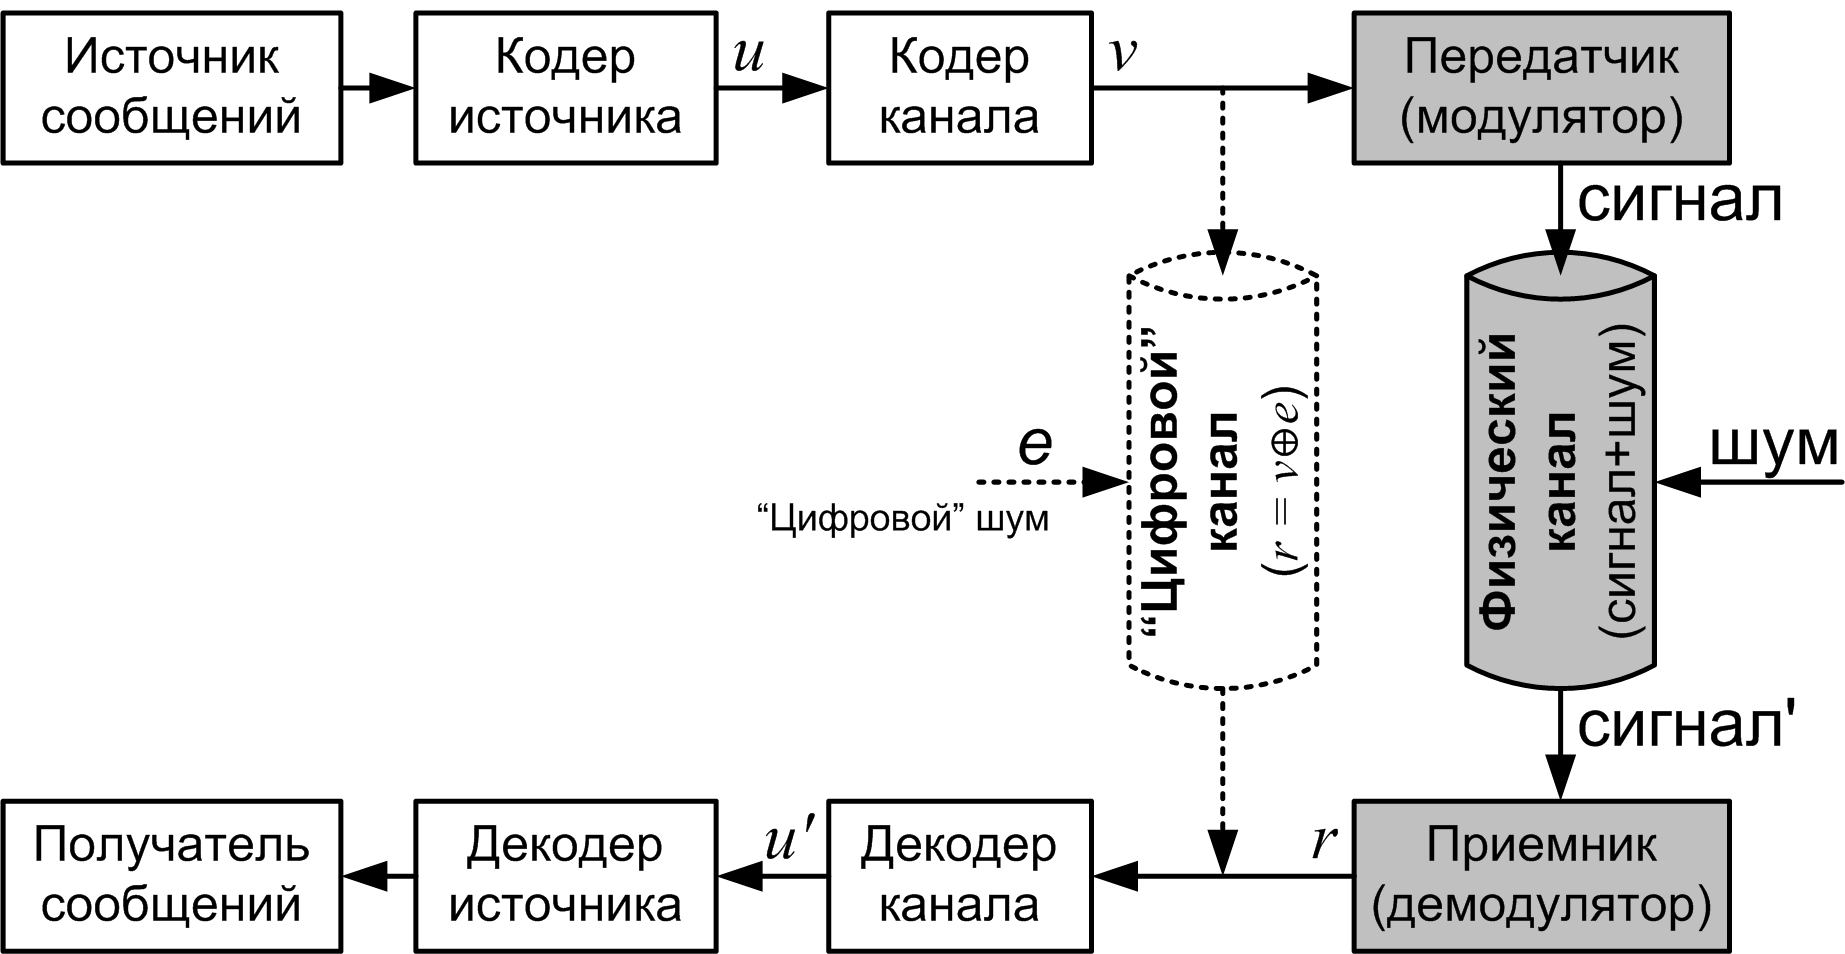
\includegraphics[width=.9\textwidth]{pict/channel} }
            \mode<article>{ 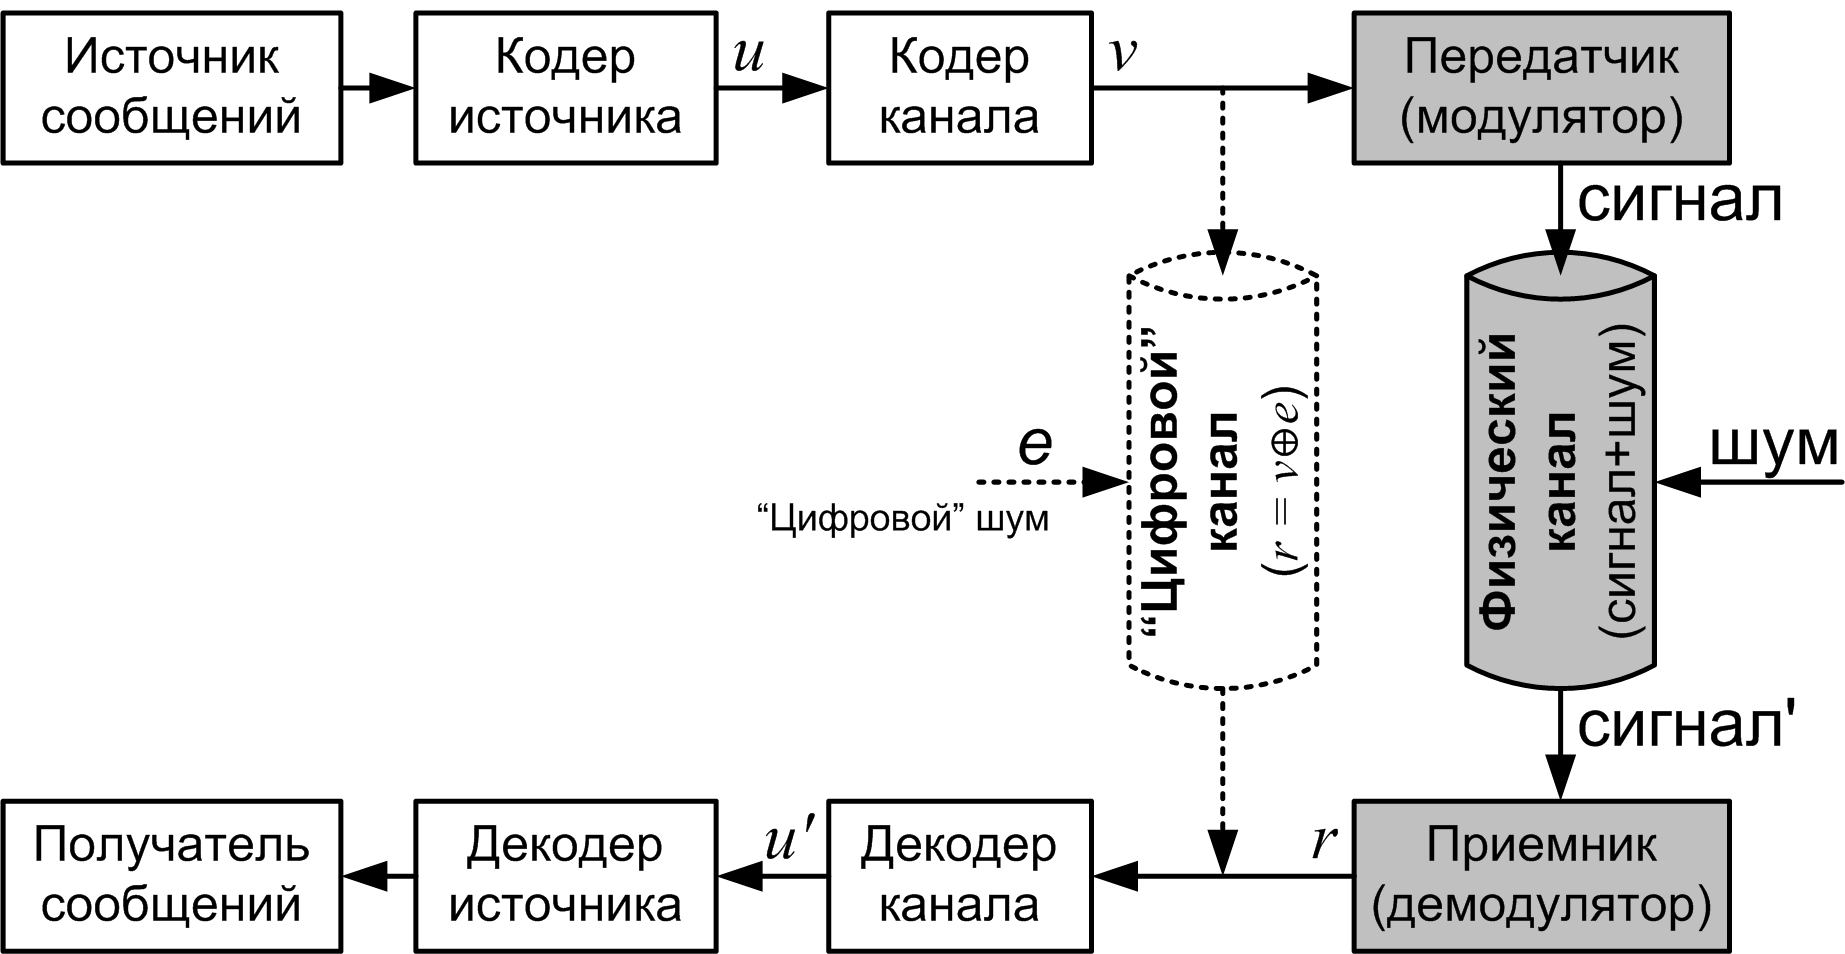
\includegraphics[width=.9\textwidth]{pict/channel} } 
            \caption{Схема канала передачи данных}\label{pict:channel}
        \end{center}
    \end{figure} 
    \mode<article>{См. Рис. \ref{pict:channel}}
\end{frame}


\begin{frame}
    \frametitle{Типы ошибок в <<цифровом>> канале}
    
    \begin{itemize}
        \item \alert{Замещение} символа\footnote{Цифры, кодового символа} (в случае двоичного кодирования --- инверсия двоичного разряда).
        
        \item Вставка символа (например, добавление бита в сообщение).
        
        \item Выпадение символа (например, исключение бита из сообщения).
    \end{itemize} 
    Далее будем рассматривать только ошибки \alert{замещения}.
\end{frame}


\begin{frame}
    \frametitle{Принципы и стратегии помехоустойчивого кодирования}
    
    Необходимо внести в исходное кодовое слово $u$ дополнительные служебные биты информации, предназначенные для повышения устойчивости к помехам. В результате исходное кодовое слово $u$ будет преобразовано кодером канала в слово $v$ большей длины.
    
    Существуют две стратегии борьбы с помехами:
    \begin{itemize}
        \item с обнаружением ошибок и с последующим запросом на повторную передачу (ARQ --- Automatic Repeat Request).
    
        \item с непосредственным обнаружением и исправлением ошибок на стороне получателя (FEC --- Forvard Error Correction);        
    \end{itemize}
    Линейные блоковые коды позволяют использовать обе стратегии.
\end{frame}


\subsection{Обозначения}


\begin{frame}
    \frametitle{Обозначения}
    Кодер ЛБК\footnote{Линейный блоковый код} переводит исходный вектор $u$ разрядности $k$ в кодовый вектор $v$ разрядности $n$. В общем случае подобный код\footnote{Так и произносится: <<эн-ка код>>} обозначают $(n, k)$. Кодером используются две двуместные операции:
    \begin{columns}
        \column{.45\textwidth}
        \begin{block}{Сложение}
            \begin{table}[ht]
                \mode<article>{\caption{Сложение}}\label{t:lbcAdd}
                \centering
                \begin{tabular}[c]{l|l|l|}
                    $\oplus$    &$0$  &$1$ \\
                    \hline
                    $0$         &$0$  &$1$ \\
                    \hline
                    $1$         &$1$  &$0$ \\
                    \hline
                \end{tabular}
            \end{table}
            \[a_0\oplus\cdots\oplus a_{n-1}=\bigoplus_{i=0}^{n-1}a_i\]
        \end{block}
        
        \column{.45\textwidth}
        \begin{block}{Умножение}
            \begin{table}[ht]
                \mode<article>{\caption{Умножение}}\label{t:lbcMul}
                \centering
                \begin{tabular}[c]{l|l|l|}
                    $\otimes$   &$0$  &$1$ \\
                    \hline
                    $0$         &$0$  &$0$ \\
                    \hline
                    $1$         &$0$  &$1$ \\
                    \hline
                \end{tabular}
            \end{table}
            \[a_0\otimes\cdots\otimes a_{n-1}=\bigotimes_{i=0}^{n-1}a_i\]
        \end{block}
        
    \end{columns}
    \mode<article>{Сложение см. \ref{t:lbcAdd}, умножение см. \ref{t:lbcMul}}
\end{frame}


\subsection{Математические основы ЛБК}


\begin{frame}
    \frametitle{Пример линейного блокового кода $(7,4)$}
    \begin{table}[ht]
        \caption{Пример линейного блокового кода $(7,4)$}\label{t:lbcExample}
        \centering
        \begin{tabular}[c]{|l|l||l|l|}
            \hline\hline
            $u$     &$v$        &$u$    &$v$\\
            \hline\hline
            0000    &000 0000   &0001   &101 0001\\
            1000    &110 1000   &1001   &011 1001\\
            0100    &011 0100   &0101   &110 0101\\
            1100    &101 1100   &1101   &000 1101\\
            0010    &111 0010   &0011   &010 0011\\
            1010    &001 1010   &1011   &100 1011\\
            0110    &100 0110   &0111   &001 0111\\
            1110    &010 1110   &1111   &111 1111\\
            \hline
        \end{tabular}
    \end{table}
    Кодовым пространством $C$ будем называть множество всех возможных кодовых векторов $v$.
    \mode<article>{См. \ref{t:lbcExample}}
\end{frame}


\begin{frame}
    \frametitle{Формирование линейного блокового кода}
    
    \begin{definition}
        Коды, в которых \alert{информационное} слово может быть непосредственно выделено из \alert{кодового} слова называются \alert{систематическими}.
    \end{definition}
    Кодирование задается порождающей матрицей $G_{k,n}$. Для приведенной выше таблицы кодирования эта матрица будет такой:
    \[
        G_{4,7} = 
            \begin{pmatrix}
                1&1&0&1&0&0&0\\
                0&1&1&0&1&0&0\\
                1&1&1&0&0&1&0\\
                1&0&1&0&0&0&1
            \end{pmatrix}
    \]
    Таким образом кодовое слово из информационного получается как $v=u\otimes G$.
\end{frame}


\begin{frame}
    \frametitle{Формирование линейного блокового кода}
    
    Например:
    \[
        v=
        \begin{pmatrix}1&0&1&0\end{pmatrix}
        \otimes
        \begin{pmatrix}
            1&1&0&1&0&0&0\\
            0&1&1&0&1&0&0\\
            1&1&1&0&0&1&0\\
            1&0&1&0&0&0&1
        \end{pmatrix}
        =
        \begin{pmatrix}0&0&1&1&0&1&0\end{pmatrix}
    \]
    Также следует обратить внимание на \alert{линейную зависимость} кодовых слов $v$. Складывая любой $v_i\oplus v_j$ обязательно получим какой либо $v_k$, принадлежащий коду. И действительно: т.к. $u_i\oplus u_j=u_k$, то, следовательно, и $(u_i\otimes G)\oplus(u_j\otimes G) = (u_i\oplus u_j)\otimes G = v_k$.
    
    Порождающую матрицу \alert{систематического} кода перестановкой столбцов и строк всегда можно привести к виду: $G_{k,n} = (P_{k,(n-k)} I_k)$.    
\end{frame}


\begin{frame}
    \frametitle{Синдромное декодирование}
    
    Порождающая матрица:
    \[
        G_{4,7} = 
            \begin{pmatrix}
                1&1&0&1&0&0&0\\
                0&1&1&0&1&0&0\\
                1&1&1&0&0&1&0\\
                1&0&1&0&0&0&1
            \end{pmatrix}
    \]
    Известно, что $v_0=u_0\oplus u_2\oplus u_3$, $v_1=u_0\oplus u_1\oplus u_2$, $v_2=u_1\oplus u_2\oplus u_3$. Так как код \alert{систематический}: $v_3=u_0$, $v_4=u_1$, $v_5=u_2$, $v_6=u_3$. Тогда справедливо (если не было ошибок), что  $v_0=v_3\oplus v_5\oplus v_6$, $v_1=v_3\oplus v_4\oplus v_5$, $v_2=v_4\oplus v_5\oplus v_6$. Или, что $s_0=r_0\oplus r_3\oplus r_5\oplus r_6=0$, $s_1=r_1\oplus r_3\oplus r_4\oplus r_5=0$, $s_2=r_2\oplus r_4\oplus r_5\oplus r_6=0$. Если в принятом кодовом слове $r$ эти равенства не выполняются ($s\neq 0$), то была ошибка.
\end{frame}


\begin{frame}
    \frametitle{Синдромное декодирование}
    
    Порождающая матрица:
    \[
        G_{4,7} = 
            \begin{pmatrix}
                1&1&0&1&0&0&0\\
                0&1&1&0&1&0&0\\
                1&1&1&0&0&1&0\\
                1&0&1&0&0&0&1
            \end{pmatrix}
    \]
    $s_0=r_0\oplus r_3\oplus r_5\oplus r_6$, $s_1=r_1\oplus r_3\oplus r_4\oplus r_5$, $s_2=r_2\oplus r_4\oplus r_5\oplus r_6$. Проверочная матрица $H_{3,7}$, такая, что $s=r\otimes (H_{3,7})^T$.
    \[
        H_{3,7} = 
            \begin{pmatrix}
                1&0&0&1&0&1&1\\
                0&1&0&1&1&1&0\\
                0&0&1&0&1&1&1
            \end{pmatrix}
    \]
    Если $G_{k,n}=\begin{pmatrix}P_{k,(n-k)}&I_k\end{pmatrix}$, то $H_{(n-k),n}=\begin{pmatrix}I_{(n-k)}&(P_{k,(n-k)})^T\end{pmatrix}$
\end{frame}


\begin{frame}
    \frametitle{Синдромное декодирование}
    
    \alert{Синдром} ошибки получается так: $s=r\otimes H^T$. 

    Справедливо, что $G\otimes H^T=0$, так как строки матрицы $G$ --- это вектора $v$. $v\otimes H^T=u\otimes G\otimes H^T=0$. Так как $r=v\oplus e$, то \[s=r\otimes H^T=(v\oplus e)\otimes H^T=e\otimes H^T.\]

    Следовательно, ненулевым синдромам можно сопоставить вектора ошибок и выполнить коррекцию (FEC). В общем случае:
    \begin{enumerate}
        \item $s=0\Leftrightarrow e\in C$.
        \begin{enumerate}
            \item $e=0$ --- ошибок не было.
            \item $e\neq 0$ --- были неисправимые ошибки.
        \end{enumerate}
        \item $s\neq 0\Leftrightarrow e\not\in C$. Ошибка будет обнаружена
            \footnote{Одиночная ошибка может быть еще и исправлена}
    \end{enumerate}
\end{frame}


\begin{frame}
    \frametitle{Линейный блоковый код}
    \framesubtitle{Алгоритм коррекции ошибок}

    \begin{enumerate}
        \item Если синдром $s=0$, то ошибок не было
            \footnote{Существует вероятность необнаружимой ошибки}.
        \item Если синдром $s\neq 0$, то исправляется\footnote{Существует возможность неверной коррекции, в случае, например, двойных ошибок} одиночная ошибка. Вектор одиночной ошибки $e$ для данного значения синдрома $s$ определяется однозначно.
    \end{enumerate}
\end{frame}


\begin{frame}
    \frametitle{Обнаружение ошибок и корректирующая способность}
    
    \begin{figure}
        \begin{center}
            \mode<presentation>{ 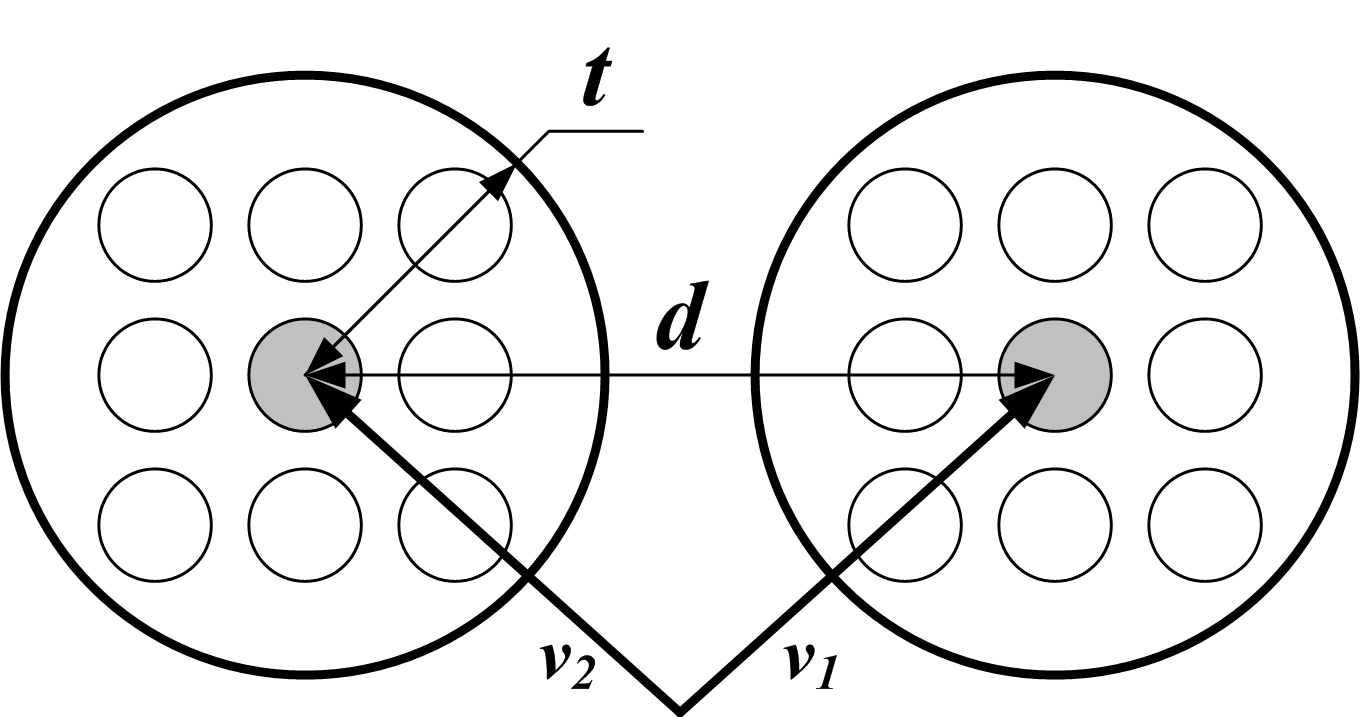
\includegraphics[width=.4\textwidth]{pict/dmin} }
            \mode<article>{ 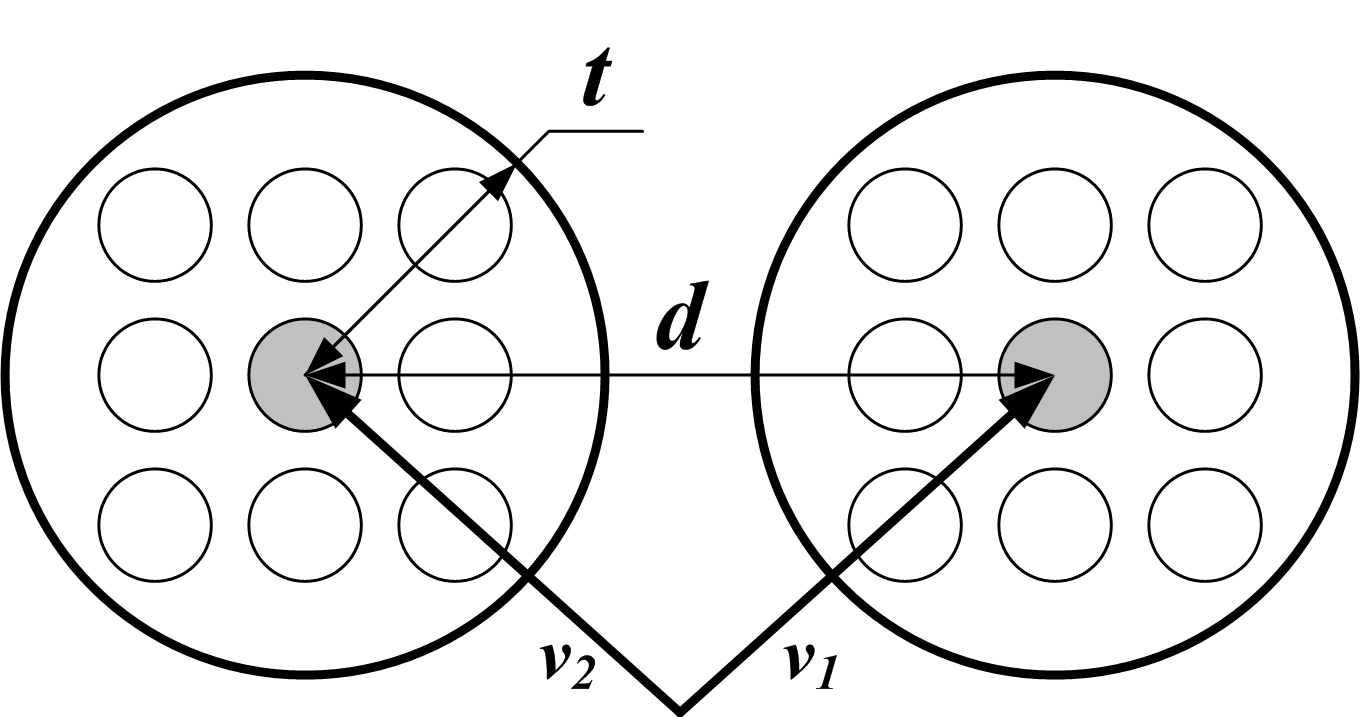
\includegraphics[width=.9\textwidth]{pict/dmin} } 
            \caption{Области декодирования}\label{pict:dmin}
        \end{center}
    \end{figure} 
    \mode<article>{См. Рис. \ref{pict:dmin}}
    \alert{Минимальное кодовое расстояние} $d_{min}$ определяется как минимальное расстояние между всеми парами кодовых векторов\footnote{В случае ЛБК $d_{min}$ определяется как количество ненулевых бит в ненулевом кодовом слове с минимальным весом} $v$. Код с минимальным кодовым расстоянием $d_{min}$ может \alert{обнаружить} $d_{min}-1$ ошибок и \alert{исправить} $t$ ошибок, где $d_{min}\geq 2t + 1$.
\end{frame}


\begin{frame}
    \frametitle{Обнаружение ошибок и корректирующая способность}
    
    Найдем взаимосвязь между параметрами двоичных $(n, k)$ кодов, способных исправлять $t$ ошибок. В этом случае не пересекающиеся сферы радиуса $t$ будут содержать все векторы, находящиеся от центра сферы на расстоянии $l$ ($0\leq l\leq t$). Таких векторов будет:
    \[ 1+n+\binom{n}{2}+\binom{n}{3}+\cdots+\binom{n}{t}=\sum_{l=0}^{t}\binom{n}{l}. \]
    
    где $\binom{n}{l}=\frac{n!}{l!\cdot(n-l)!}$. Всего сфер будет $2^k$, а всех векторов $2^n$:
    \[
        2^n\geq 2^k\cdot\sum_{l=0}^{t}\binom{n}{l}
        \ \text{или}\ 
        2^{(n-k)}\geq\sum_{l=0}^{t}\binom{n}{l}.
    \]
\end{frame}


\begin{frame}
    \frametitle{Обнаружение ошибок и корректирующая способность}
    
    В идеальном случае не пересекающиеся сферы могут содержать все вектора $n$-мерного пространства:
    \[2^{(n-k)}=\sum_{l=0}^{t}\binom{n}{l}.\]
    
    \begin{definition}
        Коды, в которых не пересекающиеся сферические области декодирования покрывают все кодовое пространство $C$ размерности $n$, называются \alert{совершенными}.
    \end{definition}
    
    Является ли приведенный в примере код совершенным?
    \uncover<2->{\[2^{(7-4)}=\binom{7}{0}+\binom{7}{1}=8\]}
\end{frame}


\section{$(n,k)$ код Хемминга}


\subsection{$(n,k)$ код Хемминга}


\begin{frame}
    \frametitle{$(n,k)$ код Хемминга}
    Коды Хемминга являются важным семейством линейных блоковых кодов\footnote{В частности, приведенный в примере линейный блоковый код является кодом Хемминга}. Для каждого натурального $m\geq 3$ можно построить код Хемминга со следующими параметрами:
    
    \begin{itemize}
        \item длина кодовых слов $n = 2^m - 1$;
        \item число информационных разрядов $k = 2^m - 1 - m$;
        \item число проверочных разрядов $m = n - k$;
        \item корректирующая способность $t=1$;
        \item минимальное кодовое расстояние $d_{min}=3$;
        \item \alert{совершенные коды}.
    \end{itemize}
\end{frame}


\subsection{Расширенный код Хемминга}


\begin{frame}
    \frametitle{Расширенный код Хемминга}
    \framesubtitle{Модификация кода Хемминга}
    
    Получаемый на выходе $(n,k)$ кодера $n$-разрядный код Хемминга $v$ дополняется слева одним битом четности. Полученный $(n+1)$-разрядный вектор $\tilde{v}$ передается в канал.
    \[
        \tilde{v}=
        \begin{pmatrix}
            \tilde{v}_0&\tilde{v}_1&\cdots&\tilde{v}_n
        \end{pmatrix}
        =
        \begin{pmatrix}
            \tilde{v}_0&v_0&v_1&\cdots&v_{n-1}
        \end{pmatrix},
    \]
    где
    \(
        \tilde{v}_0=\bigoplus_{i=0}^{n-1}v_i.
    \)
    
    Проверочная матрица $\tilde{H}_{(n-k+1),n+1}$ расширенного $(n+1,k)$ кода Хемминга получается из проверочной матрицы $H_{(n-k),n}$ так:
    \begin{enumerate}
        \item слева матрица дополняется нулевым столбцом;
        \item полученная матрица дополняется сверху строкой из единиц.
    \end{enumerate}
    При этом $\tilde{s}=\tilde{r}\otimes \tilde{H}_{(n-k+1),n+1}^T$
\end{frame}


\begin{frame}
    \frametitle{Расширенный код Хемминга}
    \framesubtitle{Пример}
    
    Видно, что \[ \tilde{s}_0=\bigoplus_{i=0}^{n}\tilde{r}_i. \]
    Например, для приведенного выше ЛБК\footnote{Код Хемминга} для вектора $v=1101000$ вектор $\tilde{v}=11101000$, а проверочная матрица
    \[
        H_{3,7} = 
            \begin{pmatrix}
                1&0&0&1&0&1&1\\
                0&1&0&1&1&1&0\\
                0&0&1&0&1&1&1
            \end{pmatrix}
        \Rightarrow
        \tilde{H}_{4,8} = 
            \begin{pmatrix}
                1&1&1&1&1&1&1&1\\
                0&1&0&0&1&0&1&1\\
                0&0&1&0&1&1&1&0\\
                0&0&0&1&0&1&1&1
            \end{pmatrix}.
    \]
\end{frame}


\begin{frame}
    \frametitle{Расширенный код Хемминга}
    \framesubtitle{Алгоритм коррекции ошибок}

    \begin{enumerate}
        \item Если синдром $\tilde{s}=0$, то ошибок не было
            \footnote{Существует вероятность необнаружимой ошибки}.
        \item Если синдром $\tilde{s}\neq 0$.
        \begin{enumerate}
            \item Если $\tilde{s}_0=1$, исправляется одиночная ошибка\footnote{Существует возможность неверной коррекции} в соответствии с синдромом $\tilde{s}$.
            \item Если $\tilde{s}_0=0$, произошла неисправимая ошибка\footnote{Можно использовать ARQ стратегию}.
        \end{enumerate}
    \end{enumerate}
\end{frame}


\begin{frame}
    \frametitle{Расширенный код Хемминга}
    Расширенные $(n,k)$ коды Хемминга являются важным расширением кодов Хемминга. Для каждого натурального $m\geq 4$ можно выделить следующие параметры:
    
    \begin{itemize}
        \item длина кодовых слов $n = 2^{m-1}$;
        \item число информационных разрядов $k = 2^{m-1} - m$;
        \item число проверочных разрядов $m = n - k$;
        \item корректирующая способность $t=1$;
        \item минимальное кодовое расстояние\footnote{Позволяет обнаруживать ошибки тройной кратности} $d_{min}=4$;
        \item обнаруживаются все ошибки нечетной кратности.
        \item \alert{совершенные коды}.
    \end{itemize}
\end{frame}


\section{$(n,k)$ циклический код}


\subsection{Двоичные многочлены}


\begin{frame}
    \frametitle{Двоичные многочлены}
    \framesubtitle{Обозначения}
    Двоичным \alert{многочленом}\footnote{Двоичным \alert{полиномом}, а далее просто многочленом или полиномом} $a(X)$ степени $n$ будем называть выражение вида 
    \[ a(X)=a_0+a_1X^1+\cdots +a_nX^n. \]
    
    Где $a_i\in \{0,1\}$ --- \alert{коэффициенты}, над которыми определены операции
    \begin{columns}
        \column{.45\textwidth}
        \begin{block}{Сложение}
            \centering
            \begin{tabular}[c]{l|l|l|}
                $\oplus$    &$0$  &$1$ \\
                \hline
                $0$         &$0$  &$1$ \\
                \hline
                $1$         &$1$  &$0$ \\
                \hline
            \end{tabular}
        \end{block}
        
        \column{.45\textwidth}
        \begin{block}{Умножение}
            \centering
            \begin{tabular}[c]{l|l|l|}
                $\otimes$   &$0$  &$1$ \\
                \hline
                $0$         &$0$  &$0$ \\
                \hline
                $1$         &$0$  &$1$ \\
                \hline
            \end{tabular}
        \end{block}
    \end{columns}
    
    \alert{Формальный символ} $X$ служит лишь для обозначения номера $i$ позиции \alert{коэффициента} $a_i$: $X^i$. Например, запись $1+X^2+X^4$ эквивалентна записи $1X^0+0X^1+1X^2+0X^3+1X^4$.
\end{frame}


\begin{frame}
    \frametitle{Двоичные многочлены}
    \framesubtitle{Операции сложения и вычитания}
    
    \alert{Сложение}
    \[a(X)+b(X)=(a_0\oplus b_0) + (a_1\oplus b_1)X + \cdots + (a_n\oplus b_n)X^n. \]
    
    \alert{Вычитание}. Так вычитание $a\ominus b$ --- это сложение с обратным элементом $-b$, таким что $b\oplus (-b)=0$, то вычитание эквивалентно сложению (так как для двоичных многочленов выходит, что $-b=b$):
    \[a(X)-b(X)=a(X)+b(X).\]
    
    Например: $(1+X+X^2)+(1+X+X^3)=X^2+X^3$.
    
\end{frame}


\begin{frame}
    \frametitle{Двоичные многочлены}
    \framesubtitle{Операция умножения}
    
    \alert{Умножение}
    \[
        \begin{split}
            a(X)b(X)=\\
            =(a_0 + \cdots + a_nX^n)(b_0 + \cdots + b_mX^m)=\\
            =c_0 + \cdots + c_{n+m}X^{n+m},
        \end{split}
    \]
    где 
    \[
        c_k=\bigoplus_{i=0}^k a_i\otimes b_{k-i}.
    \]
    
    Например: 
    \[
    \begin{split}
        (1+X+X^3)(1+X+X^2)=\\
        =(1+X+X^3)+(X+X^2+X^4)+(X^2+X^3+X^5)=\\
        =1+X^4+X^5.
    \end{split}
    \]
\end{frame}


\begin{frame}
    \frametitle{Двоичные многочлены}
    \framesubtitle{Операция деления}
    
    Результатом \alert{деления} многочлена $a(X)$ на многочлен $b(X)$ будут \alert{частное} $c(X)$ и \alert{остаток} $r(X)$, такие что 
    \[a(X)=c(X)b(X)+r(X).\]
    Причем степень $r(X)$ меньше степени $b(X)$.
\end{frame}


\begin{frame}
    \frametitle{Двоичные многочлены}
    \framesubtitle{Операция деления}
    
    Например, поделить $X^9$ на $X^4+X+1$:
    \[
        \begin{array}[c]{l|l}
            X^9 & \fbox{$X^5$}(X^4+X+1)\\
            -(X^9+X^6+X^5)&\\
            \hline
            X^6+X^5 & \fbox{$X^2$}(X^4+X+1)\\
            -(X^6+X^3+X^2)&\\
            \hline
            X^5+X^3+X^2 & \fbox{$X$}(X^4+X+1)\\
            -(X^5+X^2+X)&\\
            \hline
            \fbox{$X^3+X$} &\\
        \end{array}
    \] 
    \alert{Частное}: $X^5+X^2+X$, \alert{остаток}: $X^3+X$.
\end{frame}


\subsection{Циклический код}


Для объемов данных, используемых на практике, порождающие и проверочные матрицы линейных блоковых кодов получаются огромной размерности. Циклические коды позволяют, являясь важным подмножеством ЛБК, позволяют знечительно снизить аппаратные затраты.

В формате передачи LAPD сетей ISDN общая длина контролируемого блока (включая избыточные разряды) составляет в пределе 266 байт или 2128 бит, на контрольные разряды отводится 16 бит; потому потребуются порождающая матрица размерности 2112 x 2128 и проверочная 16 x 2128. В стандарте 802.3 требуется контролировать  целостность 1542 байт.


\begin{frame}
    \frametitle{Пример циклического кода}
    \begin{definition}
        \alert{Линейный} $(n,k)$ код является \alert{циклическим}, если циклический сдвиг любого кодового вектора $v$ из множества кодовых векторов $C$ также принадлежит $C$.
    \end{definition}
    \[
        \begin{array}[c]{c}
            v=(v_0,v_1,\ldots,v_{n-1})\\
            v^{(1)}=(v_{n-1},v_0,\ldots,v_{n-2})\\
            v^{(i)}=(v_{n-i},\ldots,v_{n-1},v_0,v_1,\ldots,v_{n-i-1})
        \end{array}
    \]
    В представлении многочленами:
    \[
        \begin{array}[c]{c}
            v(X)=v_0+v_1X+\cdots+v_{n-1}X^{n-1}\\
            v^{(1)}(X)=v_{n-1}+v_0X+\cdots+v_{n-2}X^{n-1}\\
            v^{(i)}(X)=v_{n-i}+\cdots+v_{n-1}X^{i-1}+v_0X^{i}+v_1X^{i+1}+\cdots+v_{n-i-1}X^{n-1}
        \end{array}
    \]
\end{frame}


\begin{frame}
    \frametitle{Пример циклического кода}
    \begin{table}[ht]
        \caption{Пример циклического кода}\label{t:cyclicExample}
        \centering
        \begin{tabular}[c]{|l|l||l|l|}
            \hline\hline
            $u$     &$v$        &$u$    &$v$\\
            \hline\hline
            0000    &000 0000   &0001   &101 0001\\
            1000    &110 1000   &1001   &011 1001\\
            0100    &011 0100   &0101   &110 0101\\
            1100    &101 1100   &1101   &000 1101\\
            0010    &111 0010   &0011   &010 0011\\
            1010    &001 1010   &1011   &100 1011\\
            0110    &100 0110   &0111   &001 0111\\
            1110    &010 1110   &1111   &111 1111\\
            \hline
        \end{tabular}
    \end{table}
    \mode<article>{См. табл. \ref{t:cyclicExample}}
\end{frame}


\begin{frame}
    \frametitle{Математические основы циклических кодов}
    
    \begin{theorem}
        В каждом циклическом коде существует единственный, отличный от нуля, кодовый многочлен $g(X)$ минимальной степени $r$.
    \end{theorem}

    \begin{proof}
        Допустим, что таких многочленов два: $g(X)$ и $g'(X)$. В силу линейности кода сумма этих многочленов также должна быть кодовым многочленом.
        \[
            \begin{array}[c]{c}
                g{X}=g_0+g_1X+\cdots+X^r\\
                g'(X)=g'_0+g'_1X+\cdots+X^r\\
                g(x)+g'(X)=(g_0\oplus g'_0)+(g_1\oplus g'_1)X+\cdots+(1\oplus 1)X^r
            \end{array}
        \]
    \end{proof}
\end{frame}


\begin{frame}
    \frametitle{Математические основы циклических кодов}
    
    \begin{theorem}
        Если $g(X)$ --- кодовый многочлен минимальной степени, то его коэффициент $g_0=1$.
    \end{theorem}
    
    \begin{proof}
        Предположим, что $g_0=0$
        \[
            \begin{array}[c]{c}
                g(X)=g_1X+g_2X^2+\cdots+X^r\\
                g^{(n-1)}(X)=g_1+g_2X+\cdots+X^{r-1}
            \end{array}
        \]
        Откуда следует, что $g^{(n-1)}(X)$ --- минимальный кодовый многочлен.
    \end{proof}
\end{frame}


\begin{frame}
    \frametitle{Математические основы циклических кодов}
    
    \begin{theorem}
        Пусть  $g(X)$ --- кодовый многочлен минимальной степени $r$. В этом случае, $v(X)$ является кодовым многочленом тогда и только тогда, когда он кратен g(X).
    \end{theorem}
    
    \begin{proof}
        Пусть $v(X)=a(X)g(X)$. В этом случае $(a_0 + a_1X_1 + \cdots +a_{n-1-r}X^{n-1-r})g(X)$. $v(X)$ – кодовое слово (так как это сумма кодовых слов). Пусть имеется  $v(X)$ не кратный $g(X)$. Тогда $v(X)=c(X)g(X)+b(X)$, где $b(X)$ --- остаток от деления $v(X)$ на $g(X)$. Но справедливо, что $b(X)=c(X)g(X)+v(X)$. Стало быть $b(x)$ --- кодовый многочлен степени, меньшей чем $g(X)$. Т.е. $b(X)=0$.
    \end{proof}
\end{frame}


\begin{frame}
    \frametitle{Математические основы циклических кодов}
    
    \begin{definition}
        В каждом циклическом $(n,k)$-коде существует только один многочлен минимальной степени $r=n-k$, называемый \alert{порождающим} многочленом $g(X)$, такой, что любой кодовый многочлен делится на $g(X)$. $g(X)\neq 0$
    \end{definition}
\end{frame}


\begin{frame}
    \frametitle{Математические основы циклических кодов}
    
    \begin{theorem}
        \alert{Порождающий} многочлен $g(X)$ степени $r=n-k$ циклического $(n,k)$-кода делит $X^n+1$ без остатка.
    \end{theorem}
    
    \begin{proof}
        Умножим $g(X)$ на $X^k$. Тогда получим многочлен степени $n$, такой, что через $g(X)^{(k)}$ выражается так: $g(X)X^k = g(X)^{(k)} + X^n + 1$. Причем уже доказано, что $g(X)^{(k)}=a(X)g(X)$. Тогда: $g(X)X^k = a(X)g(X) + X^n + 1$. И справедливо, что $X^n + 1 = g(X)[X^k + a(X)]$.
    \end{proof}
\end{frame}


\begin{frame}
    \frametitle{Математические основы циклических кодов}
    
    \begin{theorem}
        Если многочлен степени $n-k$ делит $X^n+1$ без остатка, то он порождает некоторый $(n,k)$-код и этот код является \alert{циклическим}.
    \end{theorem}
    
    \begin{proof}
        Всем возможным $2^k$ комбинациям информационных многочленов $u(X)$ соответствуют $v(X) = (u_0 + u_1X_1 + \cdots + u_{n-1-r}X^{n-1-r})g(X)$. Такой код является \alert{линейным}. Так как $v(X)X=v^{(1)}(X) + v_{n-1}(X^n+1)$, а $g(X)$ делит как $v(X)$ так и $X^n+1$, то он делит и $v^{(1)}(X)$. Т.е. код \alert{циклический}.
    \end{proof}
    Т.к. $X^7+1=(1+X)(1+X+X^3)(1+X^2+X^3)$, то для порождения $(7,4)$ циклического кода можно выбрать $1+X+X^3$ или $1+X^2+X^3$.
\end{frame}


\begin{frame}
    \frametitle{Систематический циклический код}
    
    Кодовый многочлен $v(X)$ \alert{циклического} кода получается из информационного многочлена $u(X)$ степени $k-1$ так:
    \[v(X)=u(X)g(X).\]
    Иногда важно\footnote{Когда проверку целостности нужно совместить с использованием $u(X)$} получить \alert{систематический} код. Для этого сдвинем $u(X)$ на $n-k$ разрядов, что эквивалентно умножению на $X^{n-k}$.
    \[
        u(X)X^{n-k}=u_0X^{n-k}+u_1X^{n-k+1}+\cdots+u_{k-1}X^{n-1}
    \]
    Поделив $u(X)X^{n-k}$ на $g(X)$ получим $u(X)X^{n-k} = a(X)g(X) + b(X)$.
    \[u(X)X^{n-k}+b(X) = a(X)g(X),\]
    где $u(X)X^{n-k}+b(X)$ --- кодовый многочлен, содержащий $u(X)$.
\end{frame}


\begin{frame}
    \frametitle{Синдромное декодирование}
    \frametitle{Связь синдрома и многочлена ошибок}
    
    \alert{Синдром} ошибки $s(X)$ получается в остатке от деления многочлена $r(X)$ на образующий $g(X)$:
    \[r(X)=a(X)g(X)+s(X).\]
    
    Так как $r(X)=v(X)+e(X)$, а $v(X)=u(X)X^r+b(x)=c(X)g(X)$, то 
    \[
        e(X)=[c(X)+a(X)]g(X)+s(X).
    \]
    Очевидно, если $e(X)$ делится на $g(X)$, то синдром будет нулевым, что соответствует \alert{необнаружимой} ошибке\footnote{Так как $e(X)\equiv s(X)\mod g(X)$, то в случае циклических кодов Хемминга можно построить однозначное соответствие между $s(X)$ и $e(X)$}.
    \[
        e(X)\equiv r(X)\mod g(X). 
    \]    
\end{frame}


\begin{frame}
    \frametitle{Пакеты ошибок}
    
    \begin{theorem}
        Если $e(X)=X^jp(X)$, где степень $p(X)$ меньше степени образующего многочлена $g(X)$, то такая ошибка будет обнаружена. 
    \end{theorem}
    
    \begin{proof}
        $e(X)=X^jp(X)$ не может делится без остатка на $g(X)$, так как в противном случае $e(X)$ было бы кодовым словом, циклический сдвиг которого давал бы кодовый многочлен минимальной степени $p(X)$, степень которого меньше $g(X)$.
    \end{proof}
\end{frame}


\begin{frame}
    \frametitle{CRC}

    CRC (Cyclic redundancy code) --- циклический избыточный код. В качестве $g(X)$ используется либо \alert{примитивный}\footnote{Примитивным двоичным многочленом степени $r$ называется многочлен $p(X)$, если $p(X)$ неразложим на множители, и минимальная степень $n$ многочлена вида $X^n+1$, делящегося на $p(X)$ без остатка, равна $n=2^r-1$} многочлен $p(X)$, либо $g(X)=(1+X)p(X)$.

    \begin{table}[ht]
        \mode<article>{\caption{CRC - коды}\label{t:crcCodes}}
        \centering
        \begin{tabular}[c]{|l|l|l|}
            \hline\hline
            Код                 &$g(X)$                         & Применение\\
            \hline\hline
            CRC-1               &$X+1$                          & Бит четности\\
            \hline
            CRC--8-CCITT        &$X^8 + X^2 + X + 1$            & ATM, HEC\\
            \hline
            CRC-16-IBM          &$X^{16} + X^{15} + X^2 + 1$    & USB\\
            \hline
            CRC--32-IEEE        &$
                                    \begin{array}[l]{l}
                                      X^{32} + X^{26} + X^{23} + X^{22} + \\
                                    + X^{16} + X^{12} + X^{11} + X^{10} + \\
                                    + X^8    + X^7    + X^5    + X^4    +\\
                                    + X^2    + X      + 1
                                    \end{array}
                                 $                                  
                                                                & Ethernet, SATA, PNG\\
            \hline
        \end{tabular}
    \end{table}
    \mode<article>{См. таблицу \ref{t:crcCodes}}
\end{frame}


\begin{frame}[fragile]
    \frametitle{CRC 32-IEEE. Инициализация}
    \framesubtitle{
        \(
            p(X)=
            X^{32} + X^{26} + X^{23} + X^{22} + 
            X^{16} + X^{12} + X^{11} + X^{10} +
            X^8    + X^7    + X^5    + X^4    +
            X^2    + X      + 1
        \)
    }
    
    Константа \verb"0xEDB88320" --- представление $p(X)$. Старший разряд константы соответствует $X^0$ и т.д., младший --- $X^{31}$.
\begin{semiverbatim}    
void InitCrcTable(unsigned int \alert{crc_table}[]) \{
    unsigned int crc, i, j;
 
    for (i = 0; i < 256; i++) \{
        for (crc = i, j = 0; j < 8; j++) \{
            if (crc & 1) \{crc = (crc {>}> 1) ^ 0xEDB88320UL;\}
            else         \{crc = crc {>}> 1;\}
        \}
        \alert{crc_table}[i] = crc;
    \}
\}
\end{semiverbatim}    
\end{frame}

\begin{frame}[fragile]
    \frametitle{CRC 32-IEEE. Табличные вычисления}
    
\begin{semiverbatim}    
unsigned int Crc32(unsigned int \alert{crc_table}[], 
                   unsigned char *buf, size_t len) \{
    unsigned int crc = 0xFFFFFFFFUL;
    
    while (len{-}-) \{
        unsigned int ch = *buf;
        crc = \alert{crc_table[}(crc ^ ch) & 0xFF\alert{]} ^ (crc {>}> 8);
        buf++;
    \}
    return crc ^ 0xFFFFFFFFUL;
\}
\end{semiverbatim}    
\end{frame}

\begin{frame}
    \frametitle{CRC}
    \framesubtitle{Характеристики}
    
    Если $g(X)=(1+X)p(X)$ и степень \alert{примитивного} многочлена $p(X)$ равна $m$, то параметры $(n,k)$ кода следующие:
    \begin{itemize}
        \item $n=2^m-1$;
        \item $k=2^m-m-2$;
        \item $d_{min}=4$;
        \item обнаруживаются ошибки четной кратности;
        \item все пакеты ошибок длины $m+1$ обнаруживаются;
        \item на практике эффективно используется в стратегии ARQ.
    \end{itemize}
\end{frame}


\subsection{Схемная реализация}


\begin{frame}
    \frametitle{Схемная реализация циклического кодирования}
    \framesubtitle{Деление на $g(X)$}
    
    \begin{figure}
        \begin{center}
            \mode<presentation>{ 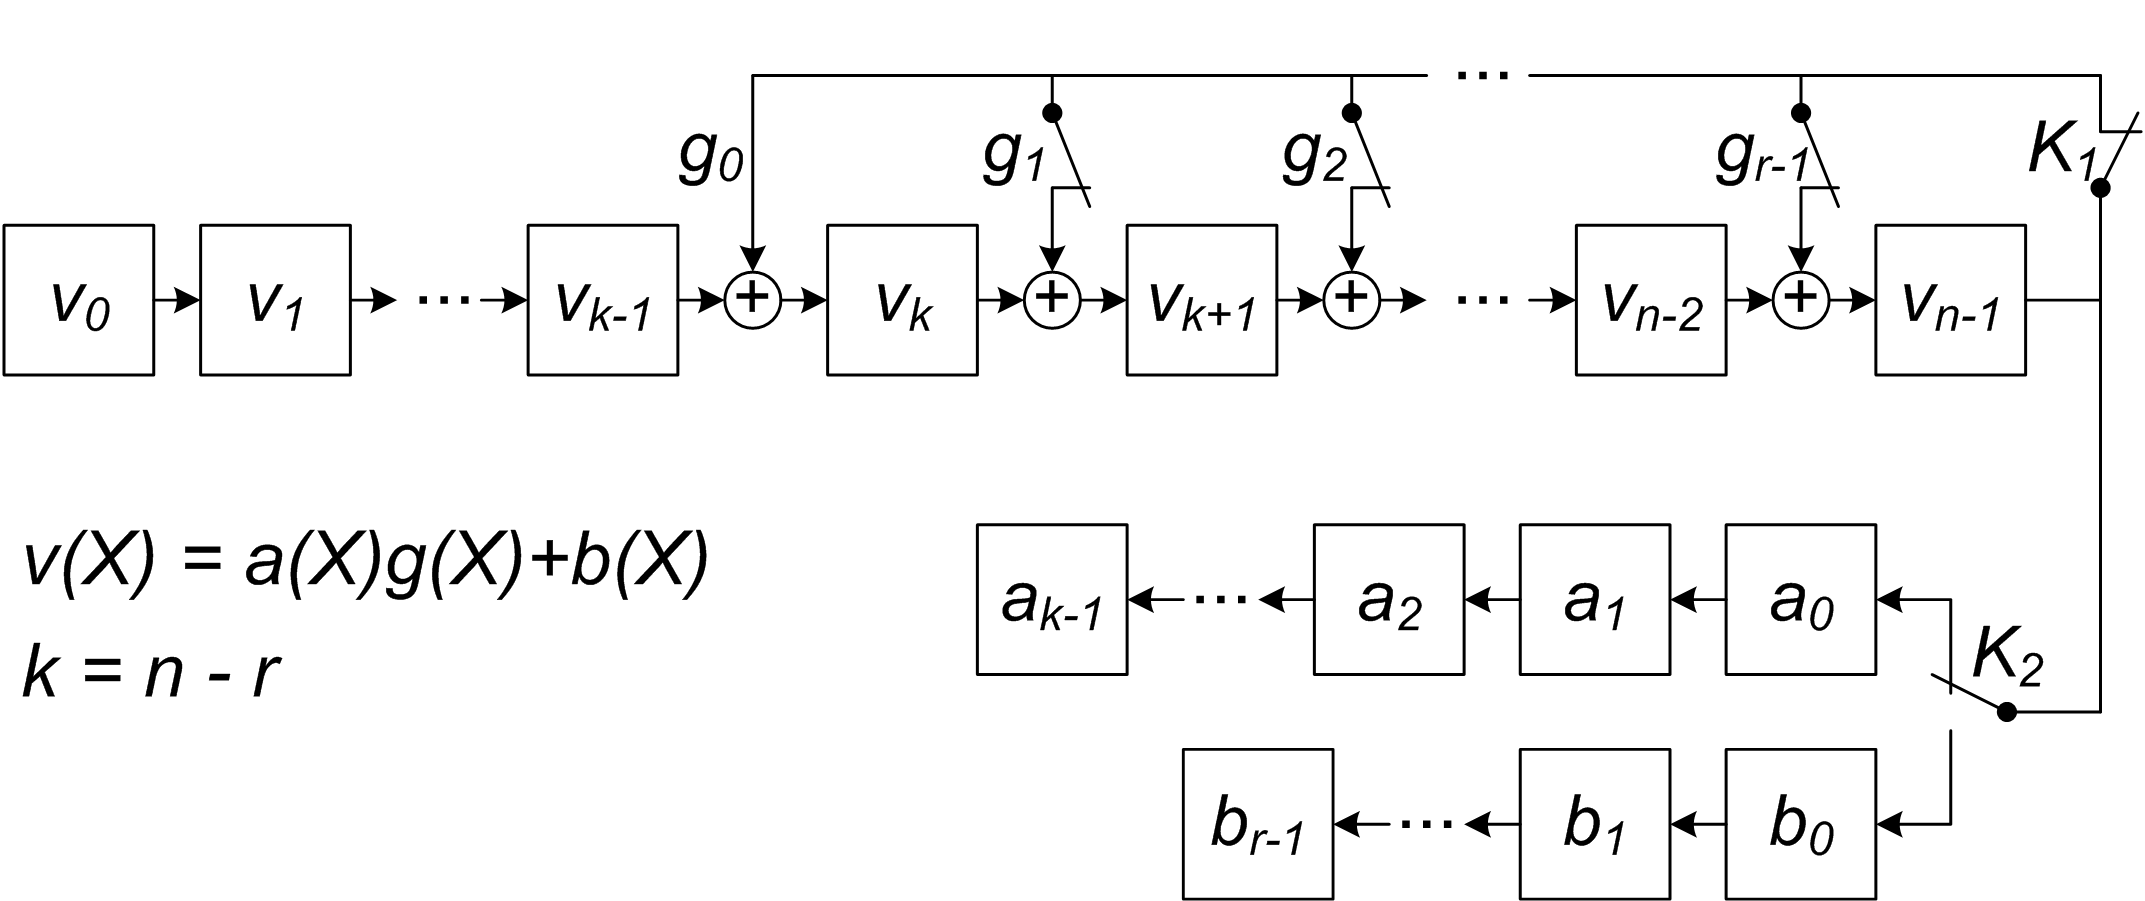
\includegraphics[width=.9\textwidth]{pict/lfsrDiv} }
            \mode<article>{ 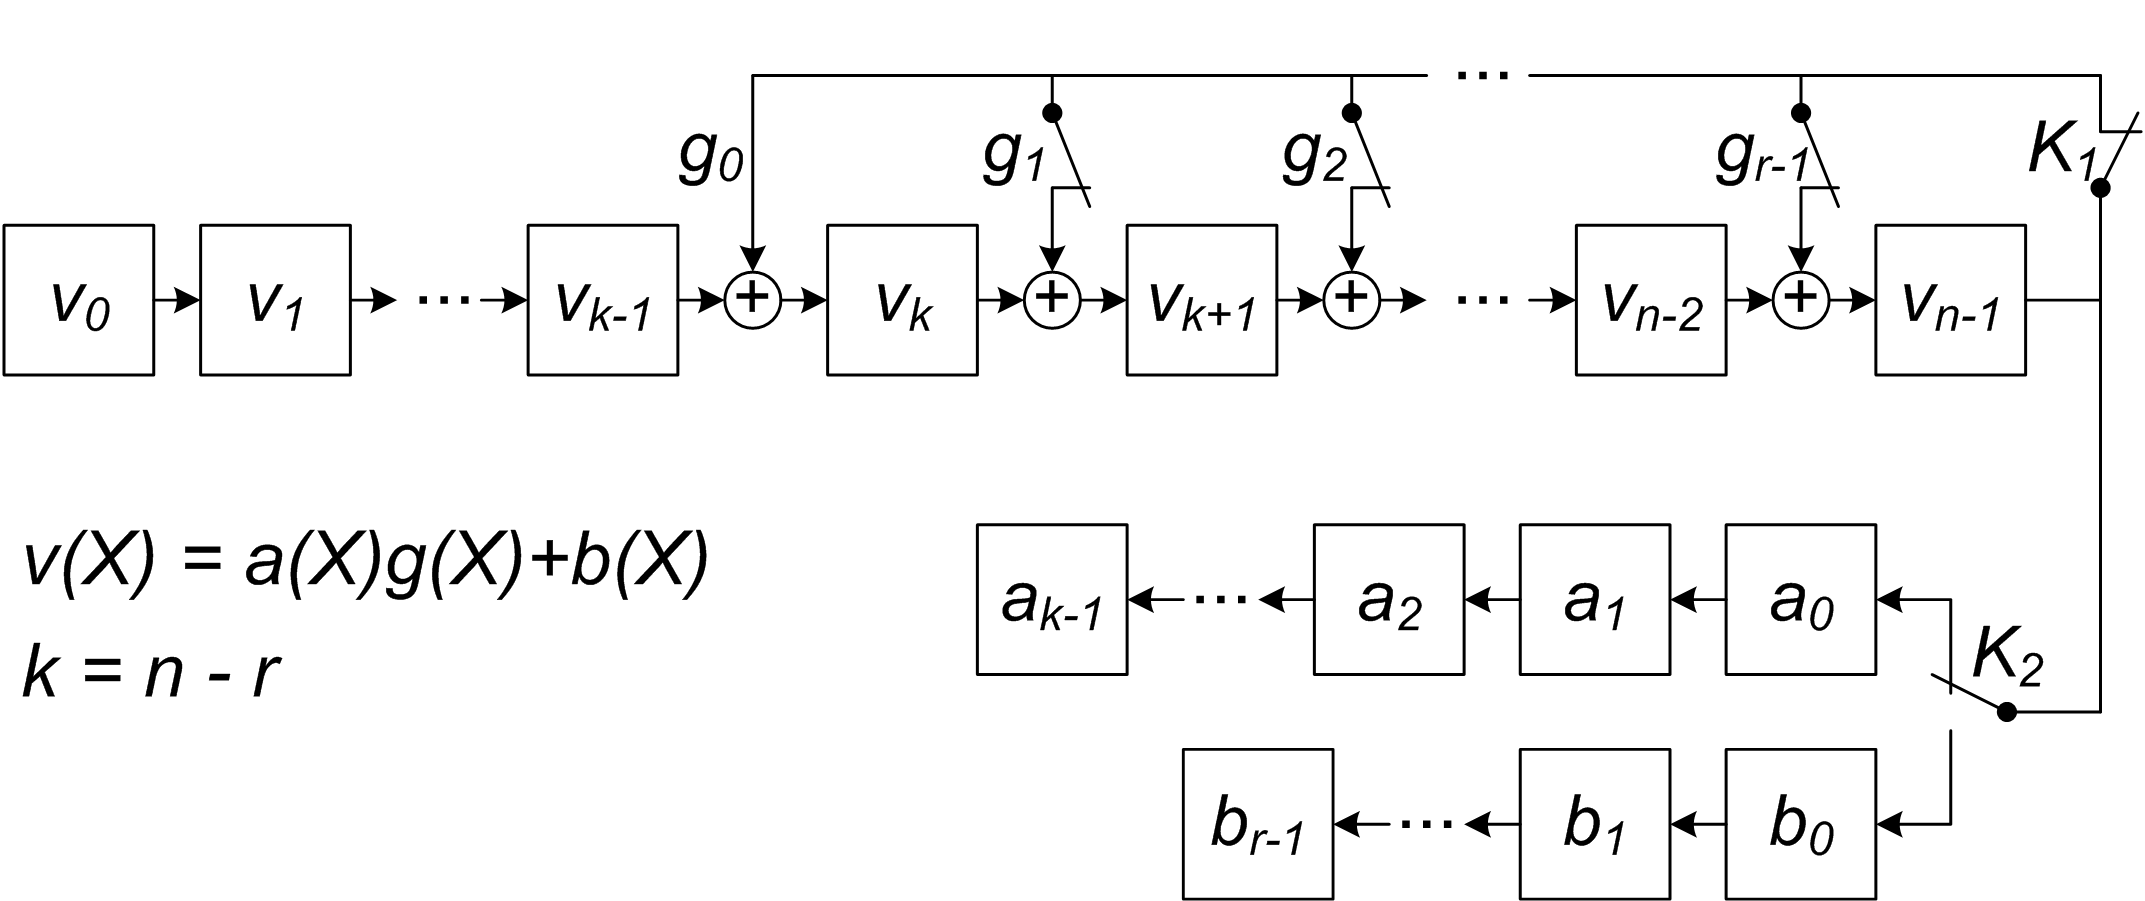
\includegraphics[width=.9\textwidth]{pict/lfsrDiv} } 
            \caption{Схема деления на $g(X)$}\label{pict:lfsrDiv}
        \end{center}
    \end{figure} 
    \mode<article>{См. Рис. \ref{pict:lfsrDiv}}
\end{frame}

Необходимо замкнуть ключ $K_1$, ключ $K_2$ поставить в верхнее положение и выполнить $k$ тактов сдвига. Таким образом в регистре $a(X)$ получается частное от деления на $g(X)$. Далее $K_1$ необходимо разомкнуть, $K_2$ перевести в нижнее положение и выполнить $r=n-k$ тактов сдвига, получая в регистре $b(X)$ остаток.

Нет необходимости получать частное $a(X)$, что несколько упрощает схемную реализацию.

\begin{frame}
    \frametitle{Схемная реализация циклического кодирования}
    \framesubtitle{Формирование систематического циклического кода}
    
    \begin{figure}
        \begin{center}
            \mode<presentation>{ 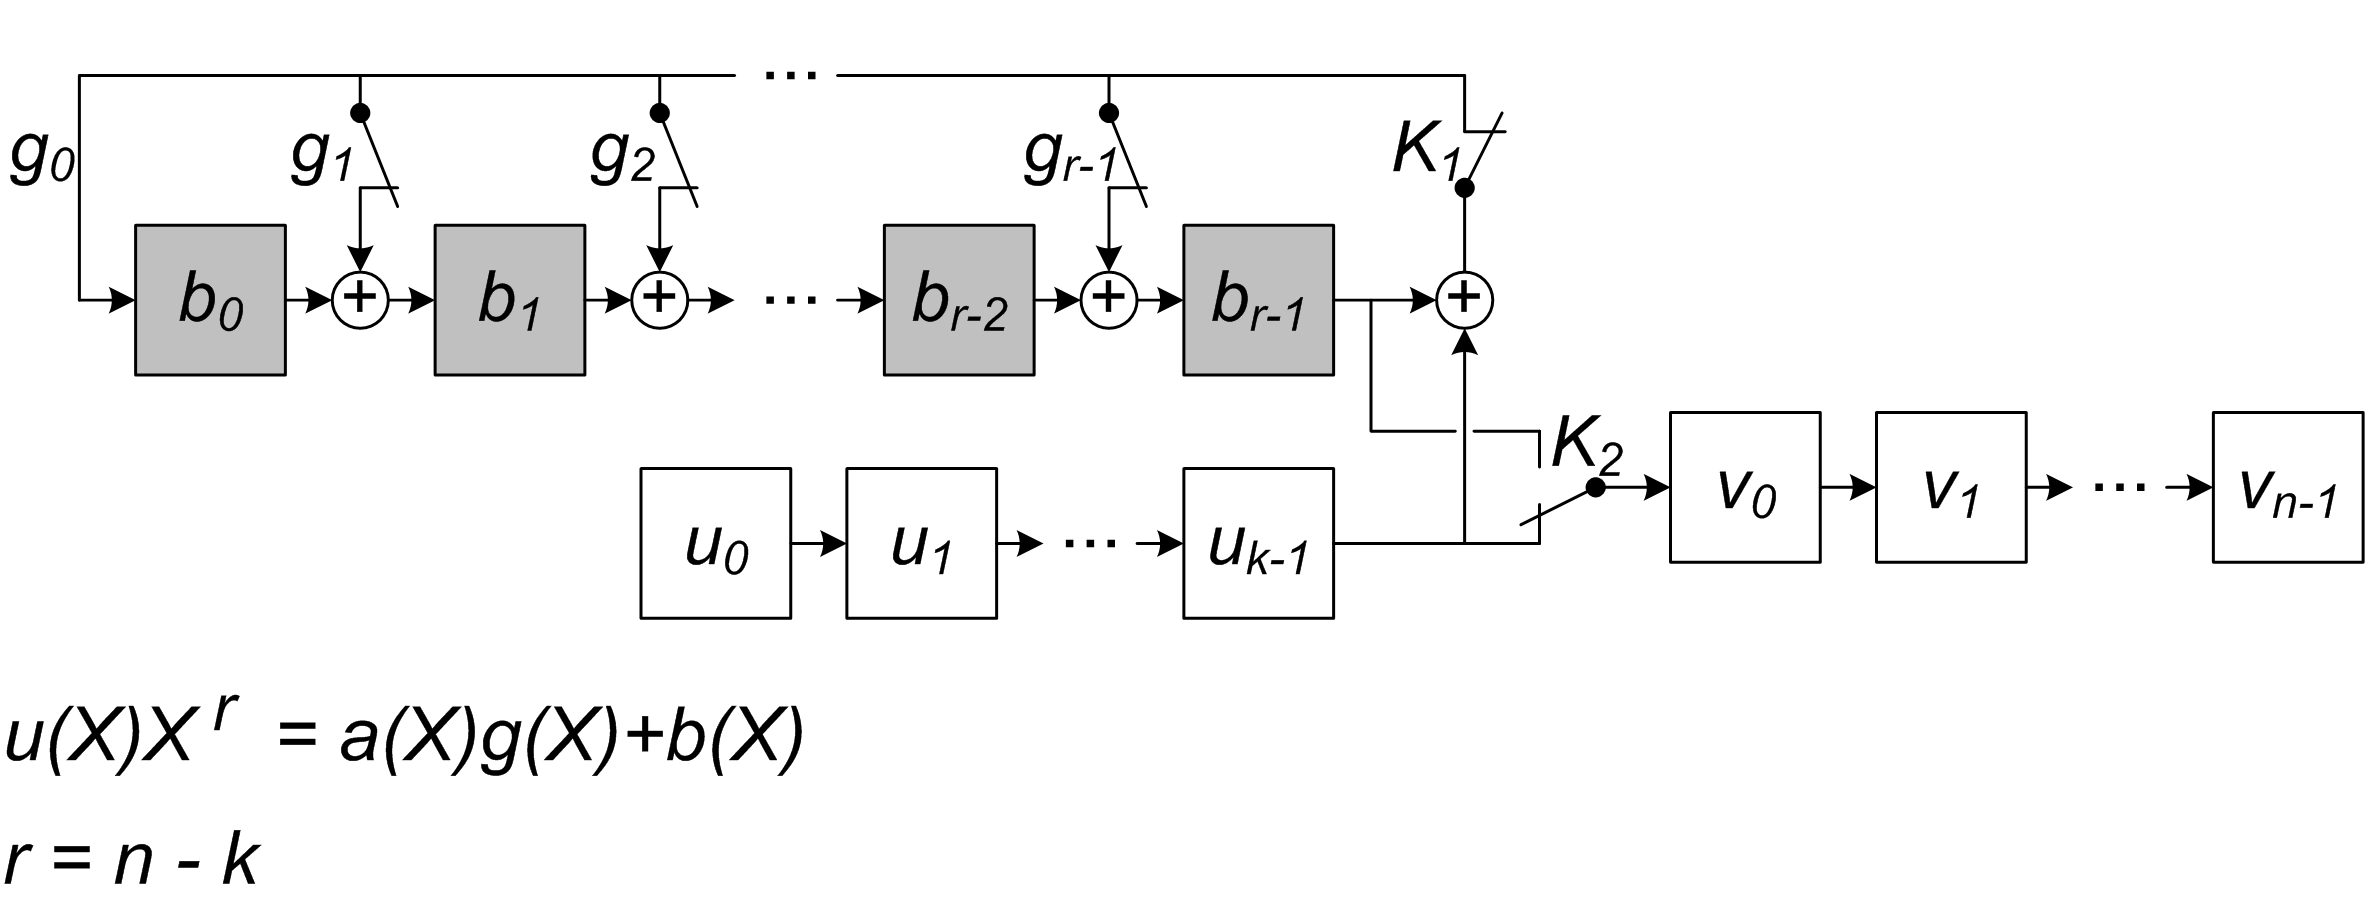
\includegraphics[width=.9\textwidth]{pict/lfsrEncode} }
            \mode<article>{ 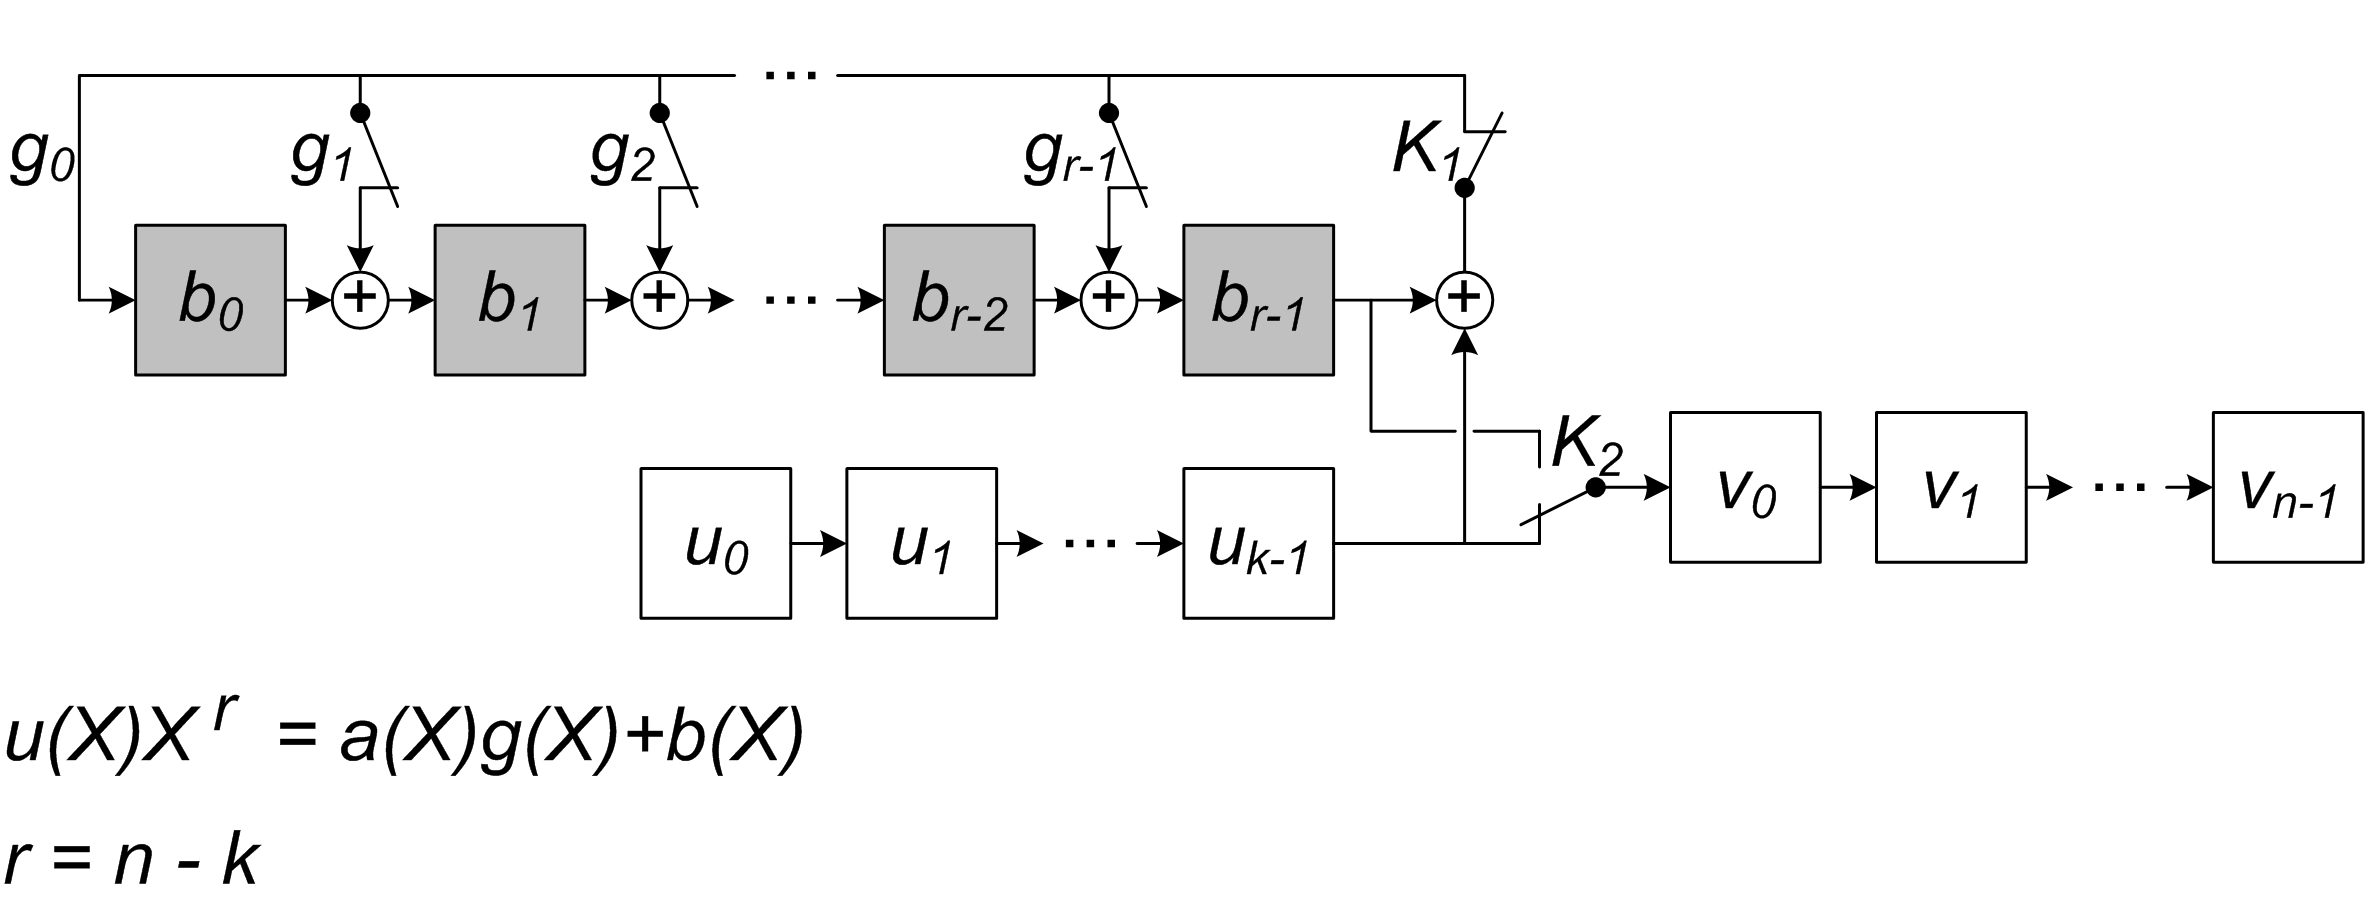
\includegraphics[width=.9\textwidth]{pict/lfsrEncode} } 
            \caption{Формирование систематического циклического кода}\label{pict:lfsrEncode}
        \end{center}
    \end{figure} 
    \mode<article>{См. Рис. \ref{pict:lfsrEncode}}
\end{frame}

В разряды $b_0\cdots b_{r-1}$ нужно записать нули. Ключ $K_1$ необходимо замкнуть, а ключ $K_2$ поставить в нижнее положение. Выполнить $k$ тактов сдвига, что приведет к тому, что $u(X)$ будет перенесен в младшие разряды $v(X)$, а в разрядах $b(X)$ будет получен остаток от деления $u(X)X^r$ на $g(X)$. Далее осталось разомкнуть ключ $K_1$, первести ключ $K_2$ в верхнее положение и, выполнив $r=n-k$ тактов, перенести остаток в младшие разряды $v(X)$.

\begin{frame}
    \frametitle{Схемная реализация циклического кодирования}
    \framesubtitle{Синдромное декодирование}
    
    \begin{figure}
        \begin{center}
            \mode<presentation>{ 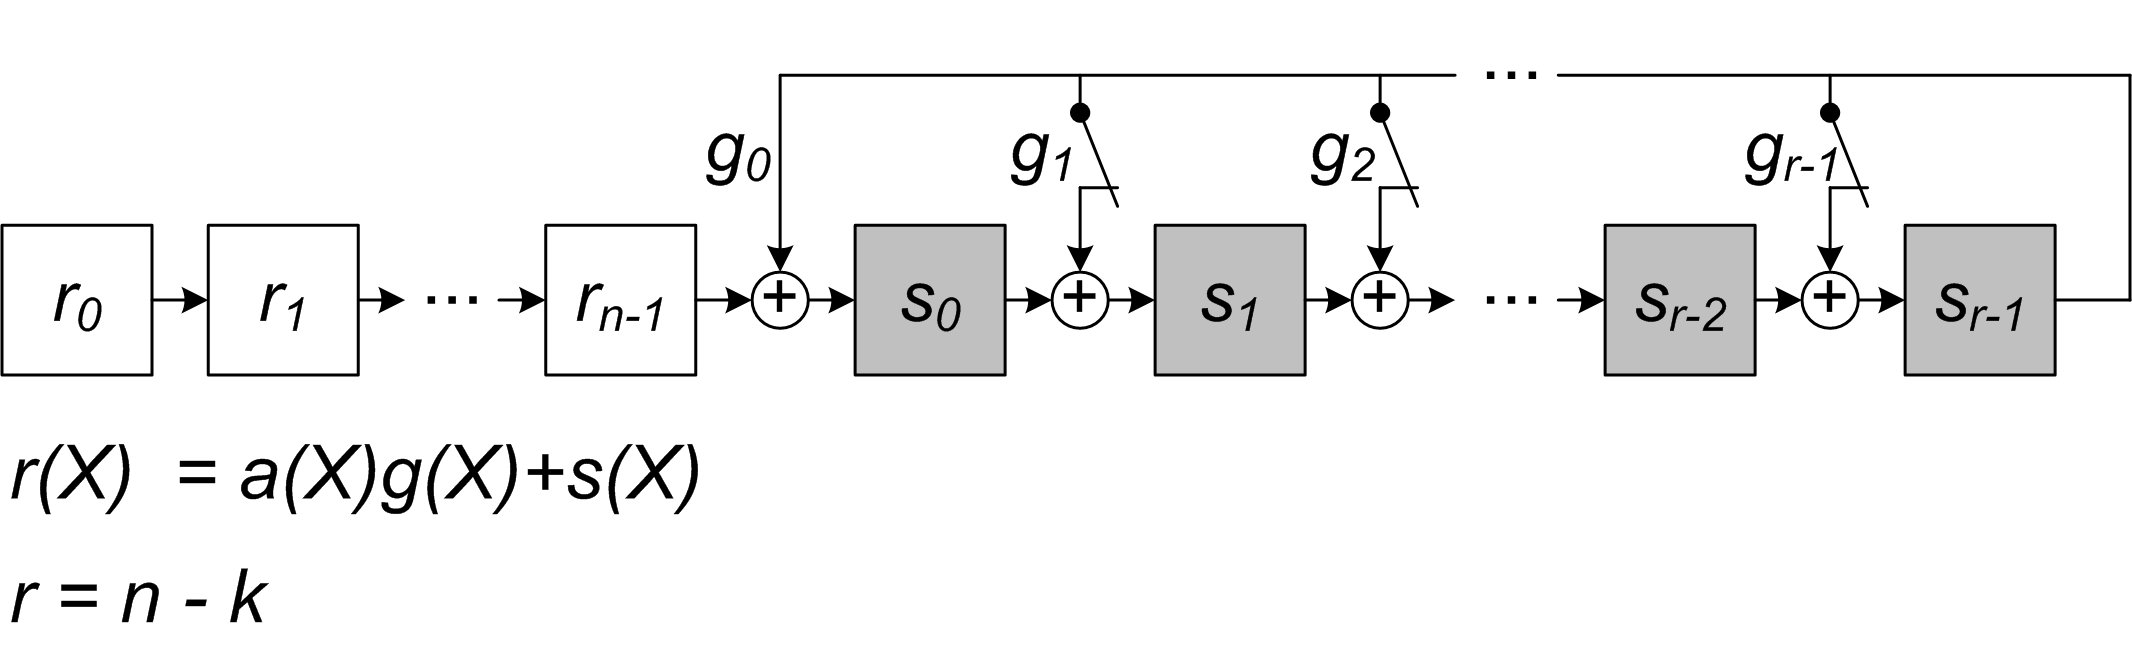
\includegraphics[width=.9\textwidth]{pict/lfsrDecode} }
            \mode<article>{ 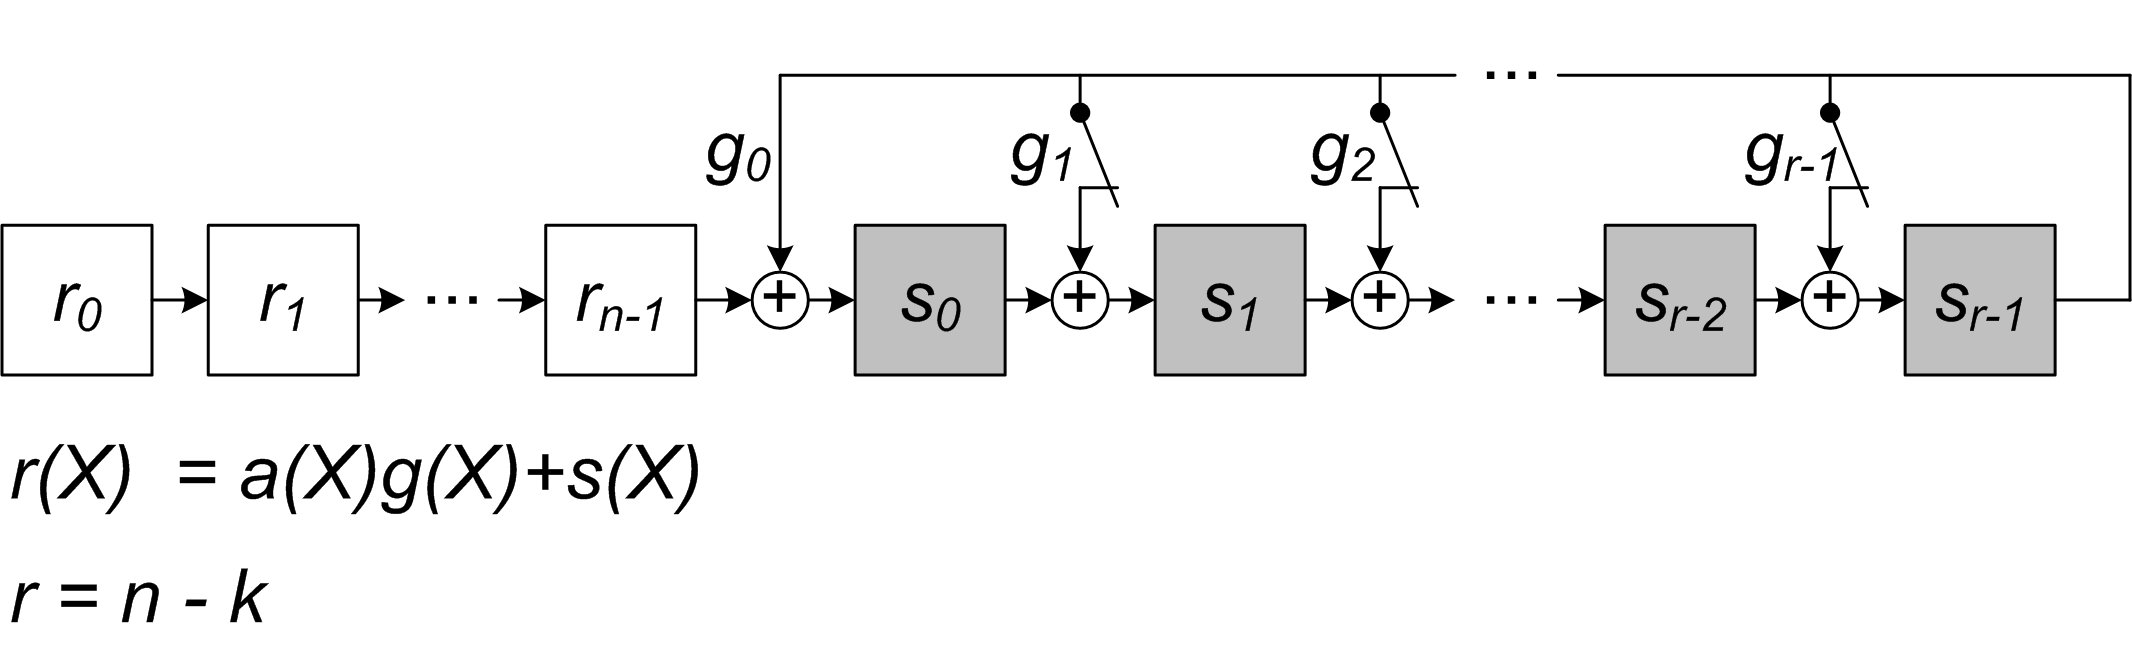
\includegraphics[width=.9\textwidth]{pict/lfsrDecode} } 
            \caption{Синдромное декодирование}\label{pict:lfsrDecode}
        \end{center}
    \end{figure} 
    \mode<article>{См. Рис. \ref{pict:lfsrDecode}}
\end{frame}

Здесь достаточно проинициализировать разряды $s(X)$ нулями и выполнить $n$ тактов сдвига. Получаемый в результате ненулевой $s(X)$ будет свидетельствовать о возникновении ошибок.

\appendix %примечания


\begin{frame}
    \frametitle{Источники}
    
    Предметное обсуждение помехоустойчивого кодирования (включая коды Хемминга, циклические и свёрточные коды) можно найти в \cite{bib:verner:codingBase}.
    
    Математические основы помехоустойчивого кодирования изложены в \cite{bib:novic:discrmathprogrammer,bib:yablonsky:discreteintro}.
\end{frame}


\begin{frame}[allowframebreaks]{Библиография}
    \bibliographystyle{gost780u}
    \bibliography{./../bibliobase}
\end{frame}

\end{document}